\section*{Results and discussion}

Using data from a previous study of the corticospinal tract profile and ALS\cite{sarica2017corticospinal}, we tested the performance of AFQ-Insight in a classification setting. The previous study predicted ALS status with a mean accuracy of 80\% using a random forest algorithm based on a priori selection of features within the corticospinal tract. AFQ-Insight delivers competitive predictive performance (mean 84\% accuracy, 0.93 ROC AUC) without the need for a priori feature engineering. The results of the classification prediction are shown in Fig~\ref{fig:class-results}, with ``ground-truth'' ALS status separated into columns, and predicted ALS status encoded by color. In addition to this classification performance, AFQ Insight also identifies the white matter tracts most important for the ALS classification. The relative importance of white matter features is captured in the $\beta$ coefficients from Eq~\eqref{eq:sgl}. Fig~\ref{fig:class-beta} depicts these coefficients ``unfolded'' across the brain. The $x$-axis organizes white matter tracts starting with left distal tracts, progressing toward the center of the brain and then outward toward the right distal tracts. Fig~\ref{fig:class-beta} shows that AFQ-Insight selects FA metrics in the right corticospinal tract as most important to ALS classification, confirming previous findings\cite{van2011upper, toosy2003diffusion, sarica2014tractography, sage2007quantitative, sage2009quantitative, karlsborg2004corticospinal, ellis1999diffusion, cosottini2005diffusion, ciccarelli2009investigation, abe2010voxel} and identifying exactly the portions of the brain that were selected \emph{a priori} in the previous study from which we collected our data\cite{sarica2017corticospinal}.

\begin{figure}[!h]
    \centering
    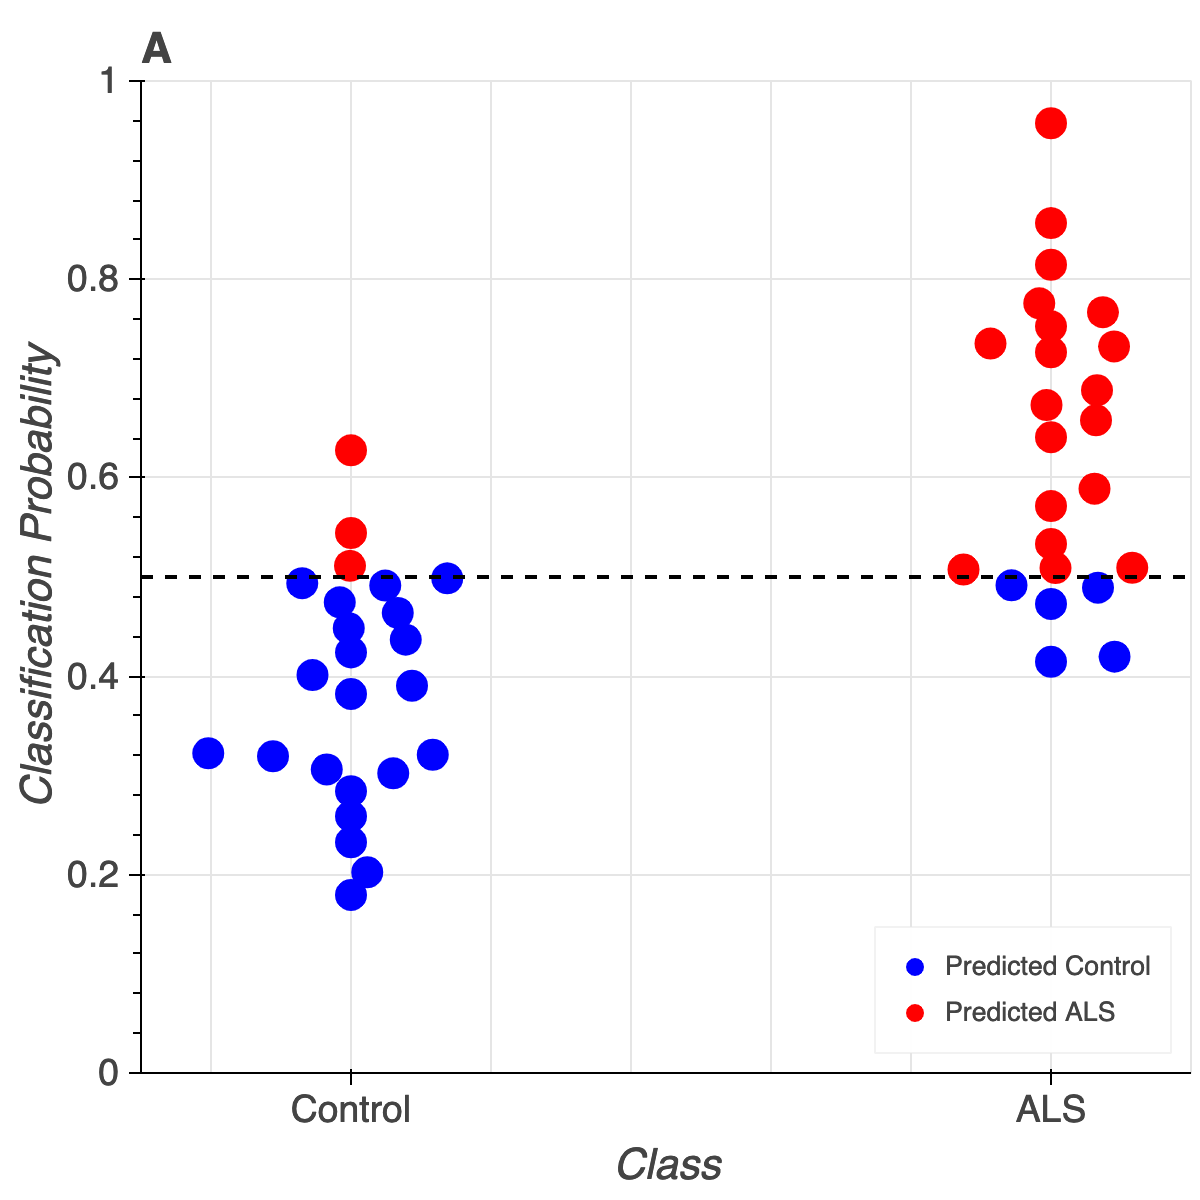
\includegraphics[width=0.65\textwidth]{classification_results.png}
    \caption{{\bf Prediction of ALS status.}
        Classification probabilities for each subject's ALS diagnosis. Controls are on the left while patients are on the right. Predicted controls are in blue and predicted patients are in red. Thus, false positive are represented as red dots on the left, while false negatives are represented as blue dots on the right. AFQ-Insight achieves 84\% accuracy with an ROC area under the curve of 0.93.
    }
    \label{fig:class-results}
\end{figure}

\begin{figure}[!h]
    \centering
    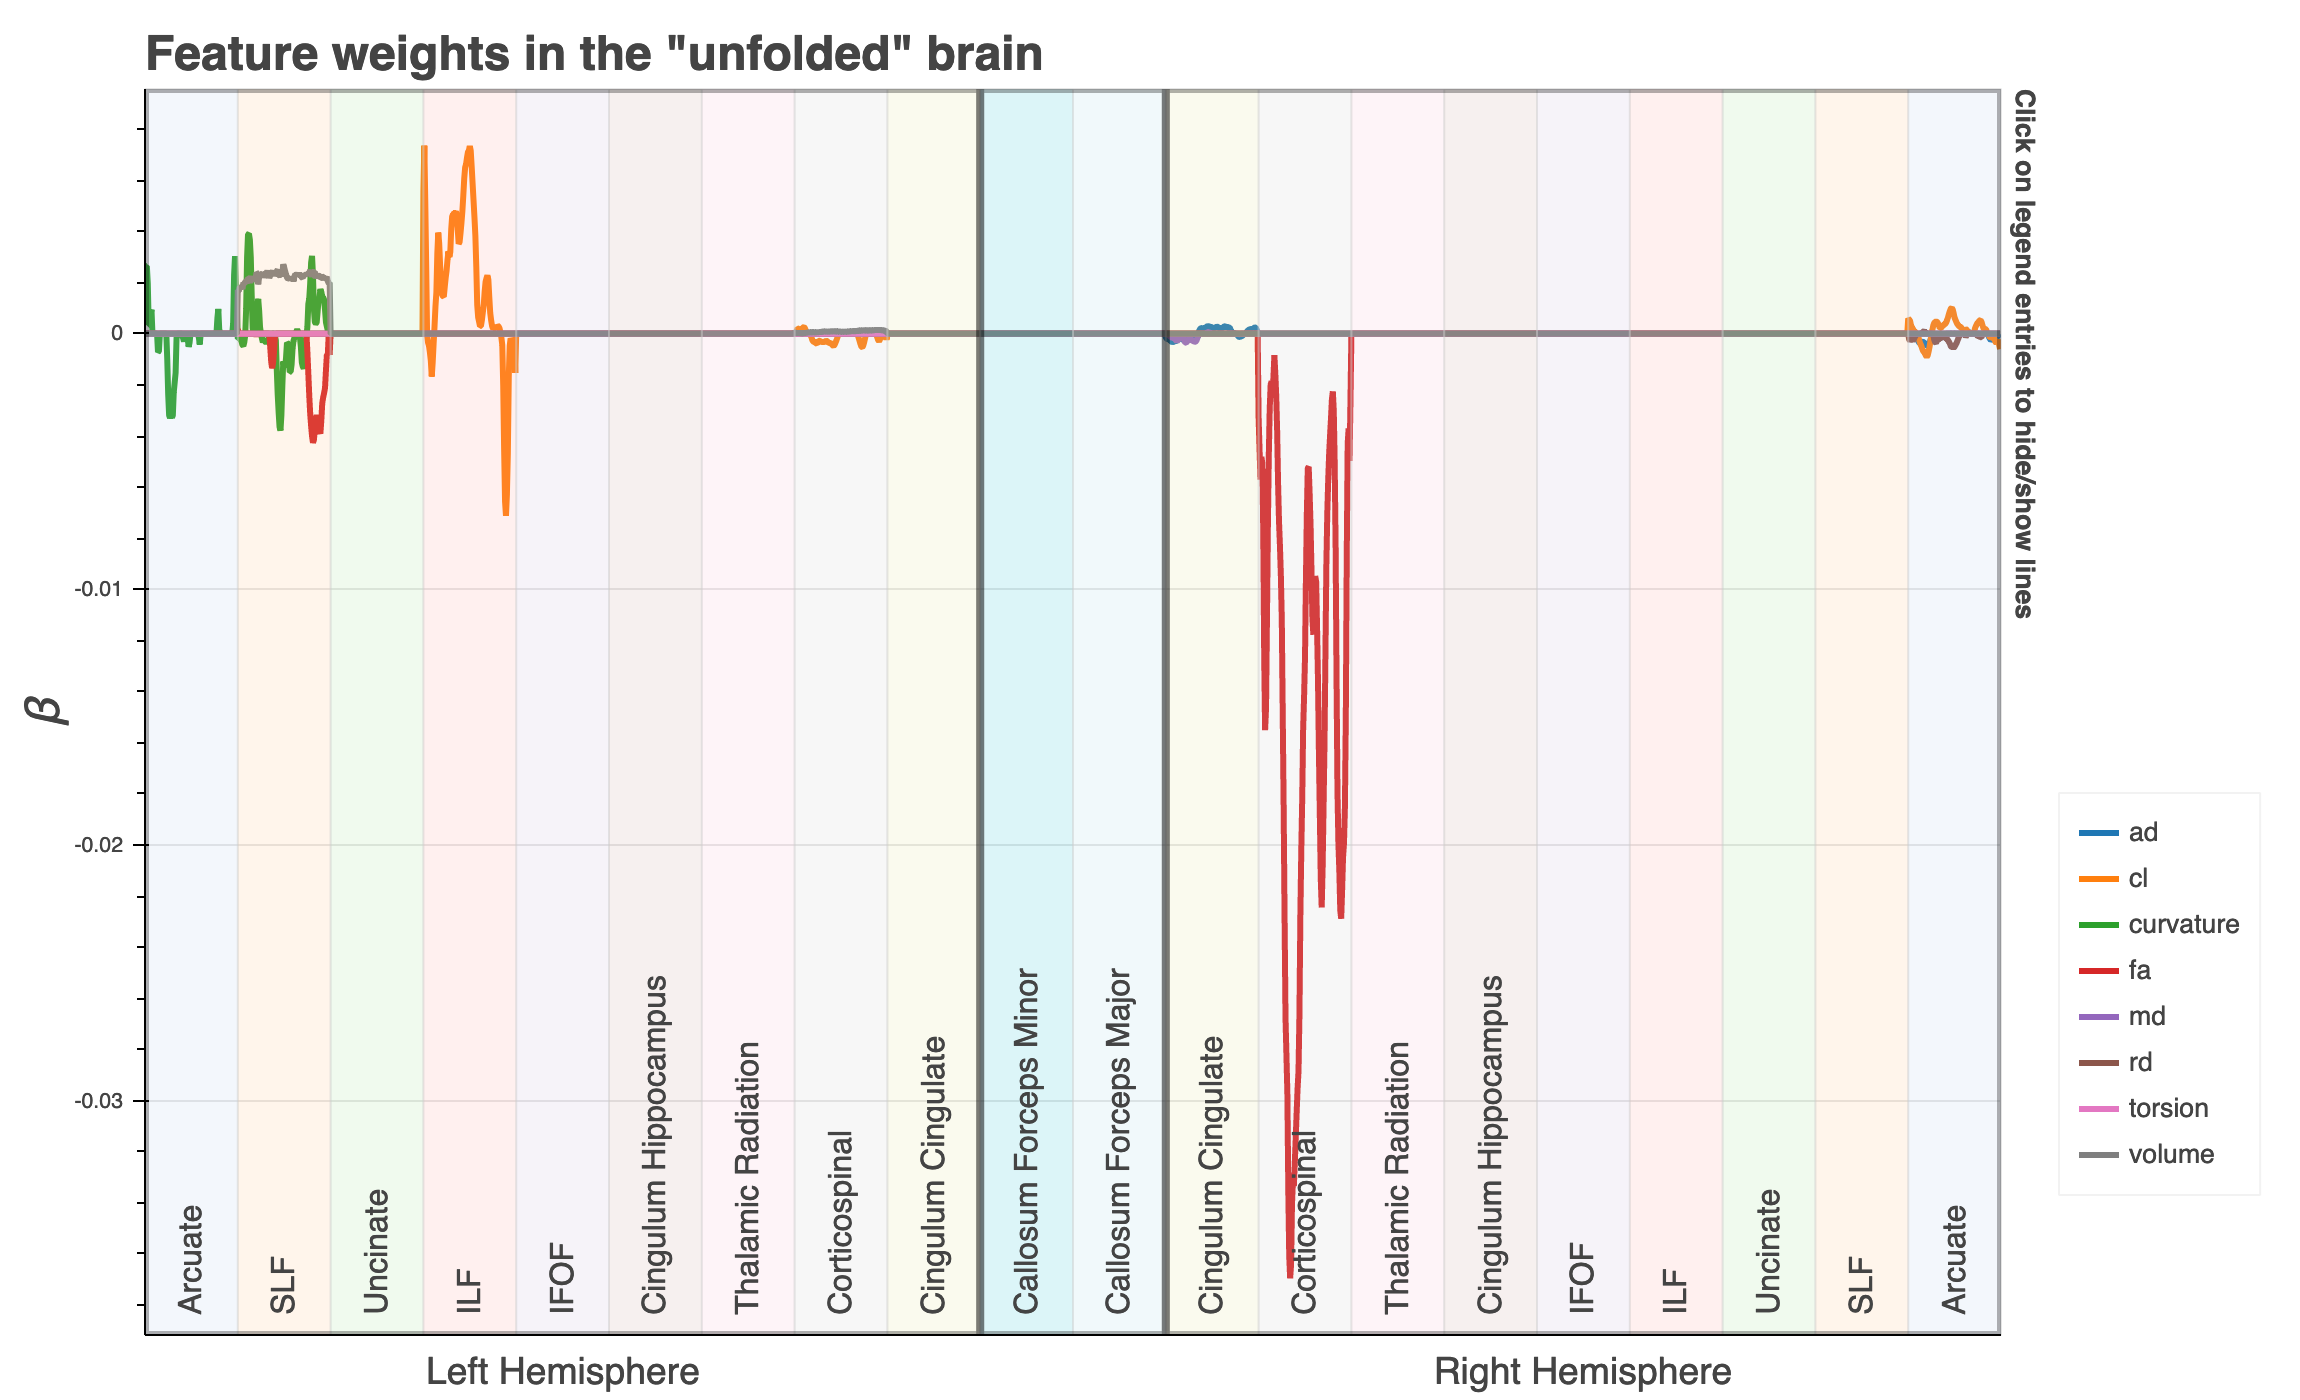
\includegraphics[width=0.95\textwidth]{classification_unfolded_beta.png}
    \caption{{\bf Feature importance for prediction of ALS status.}
        Classification probabilities for each subject's ALS diagnosis. Controls are on the left while patients are on the right. Predicted controls are in blue and predicted patients are in red. Thus, false positive are represented as red dots on the left, while false negatives are represented as blue dots on the right. AFQ-Insight achieves 84\% accuracy with an ROC area under the curve of 0.93.
    }
    \label{fig:class-beta}
\end{figure}

\begin{itemize}
  \item Classification
    \begin{itemize}
      \item Insert figure showing weights as they relate to tract differences visible in the browser
    \end{itemize}
\end{itemize}

In a regression setting, we attempted to accurately predict ``brain age''.

\begin{figure}[!h]
    \centering
    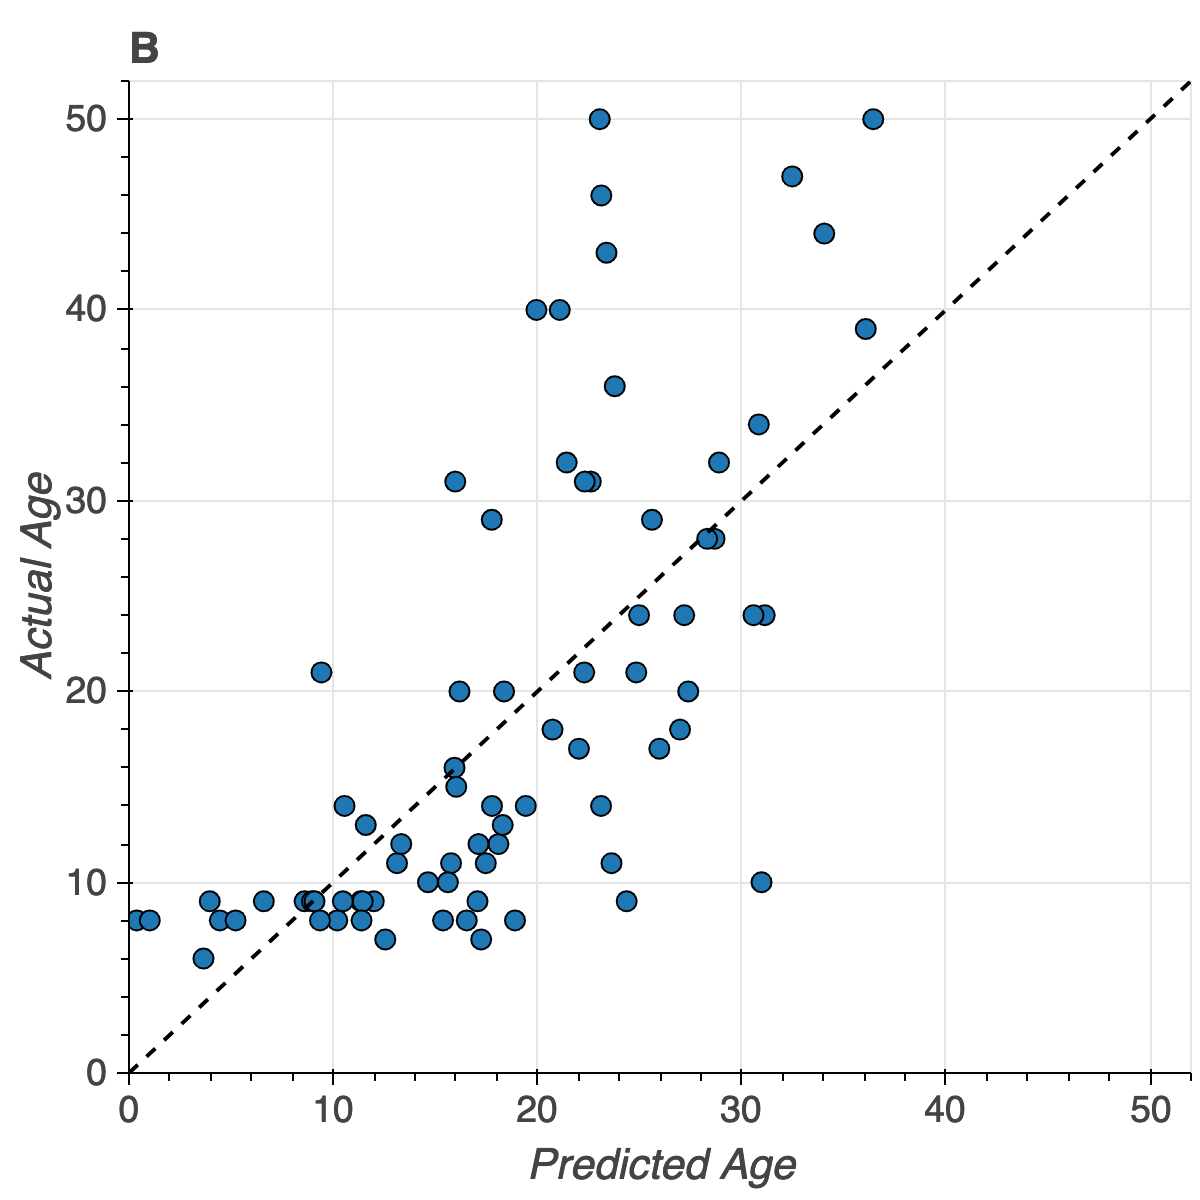
\includegraphics[width=0.65\textwidth]{regression_results.png}
    \caption{{\bf Prediction of brain age.}
    }
    \label{fig:regress-results}
\end{figure}

\begin{figure}[!h]
    \centering
    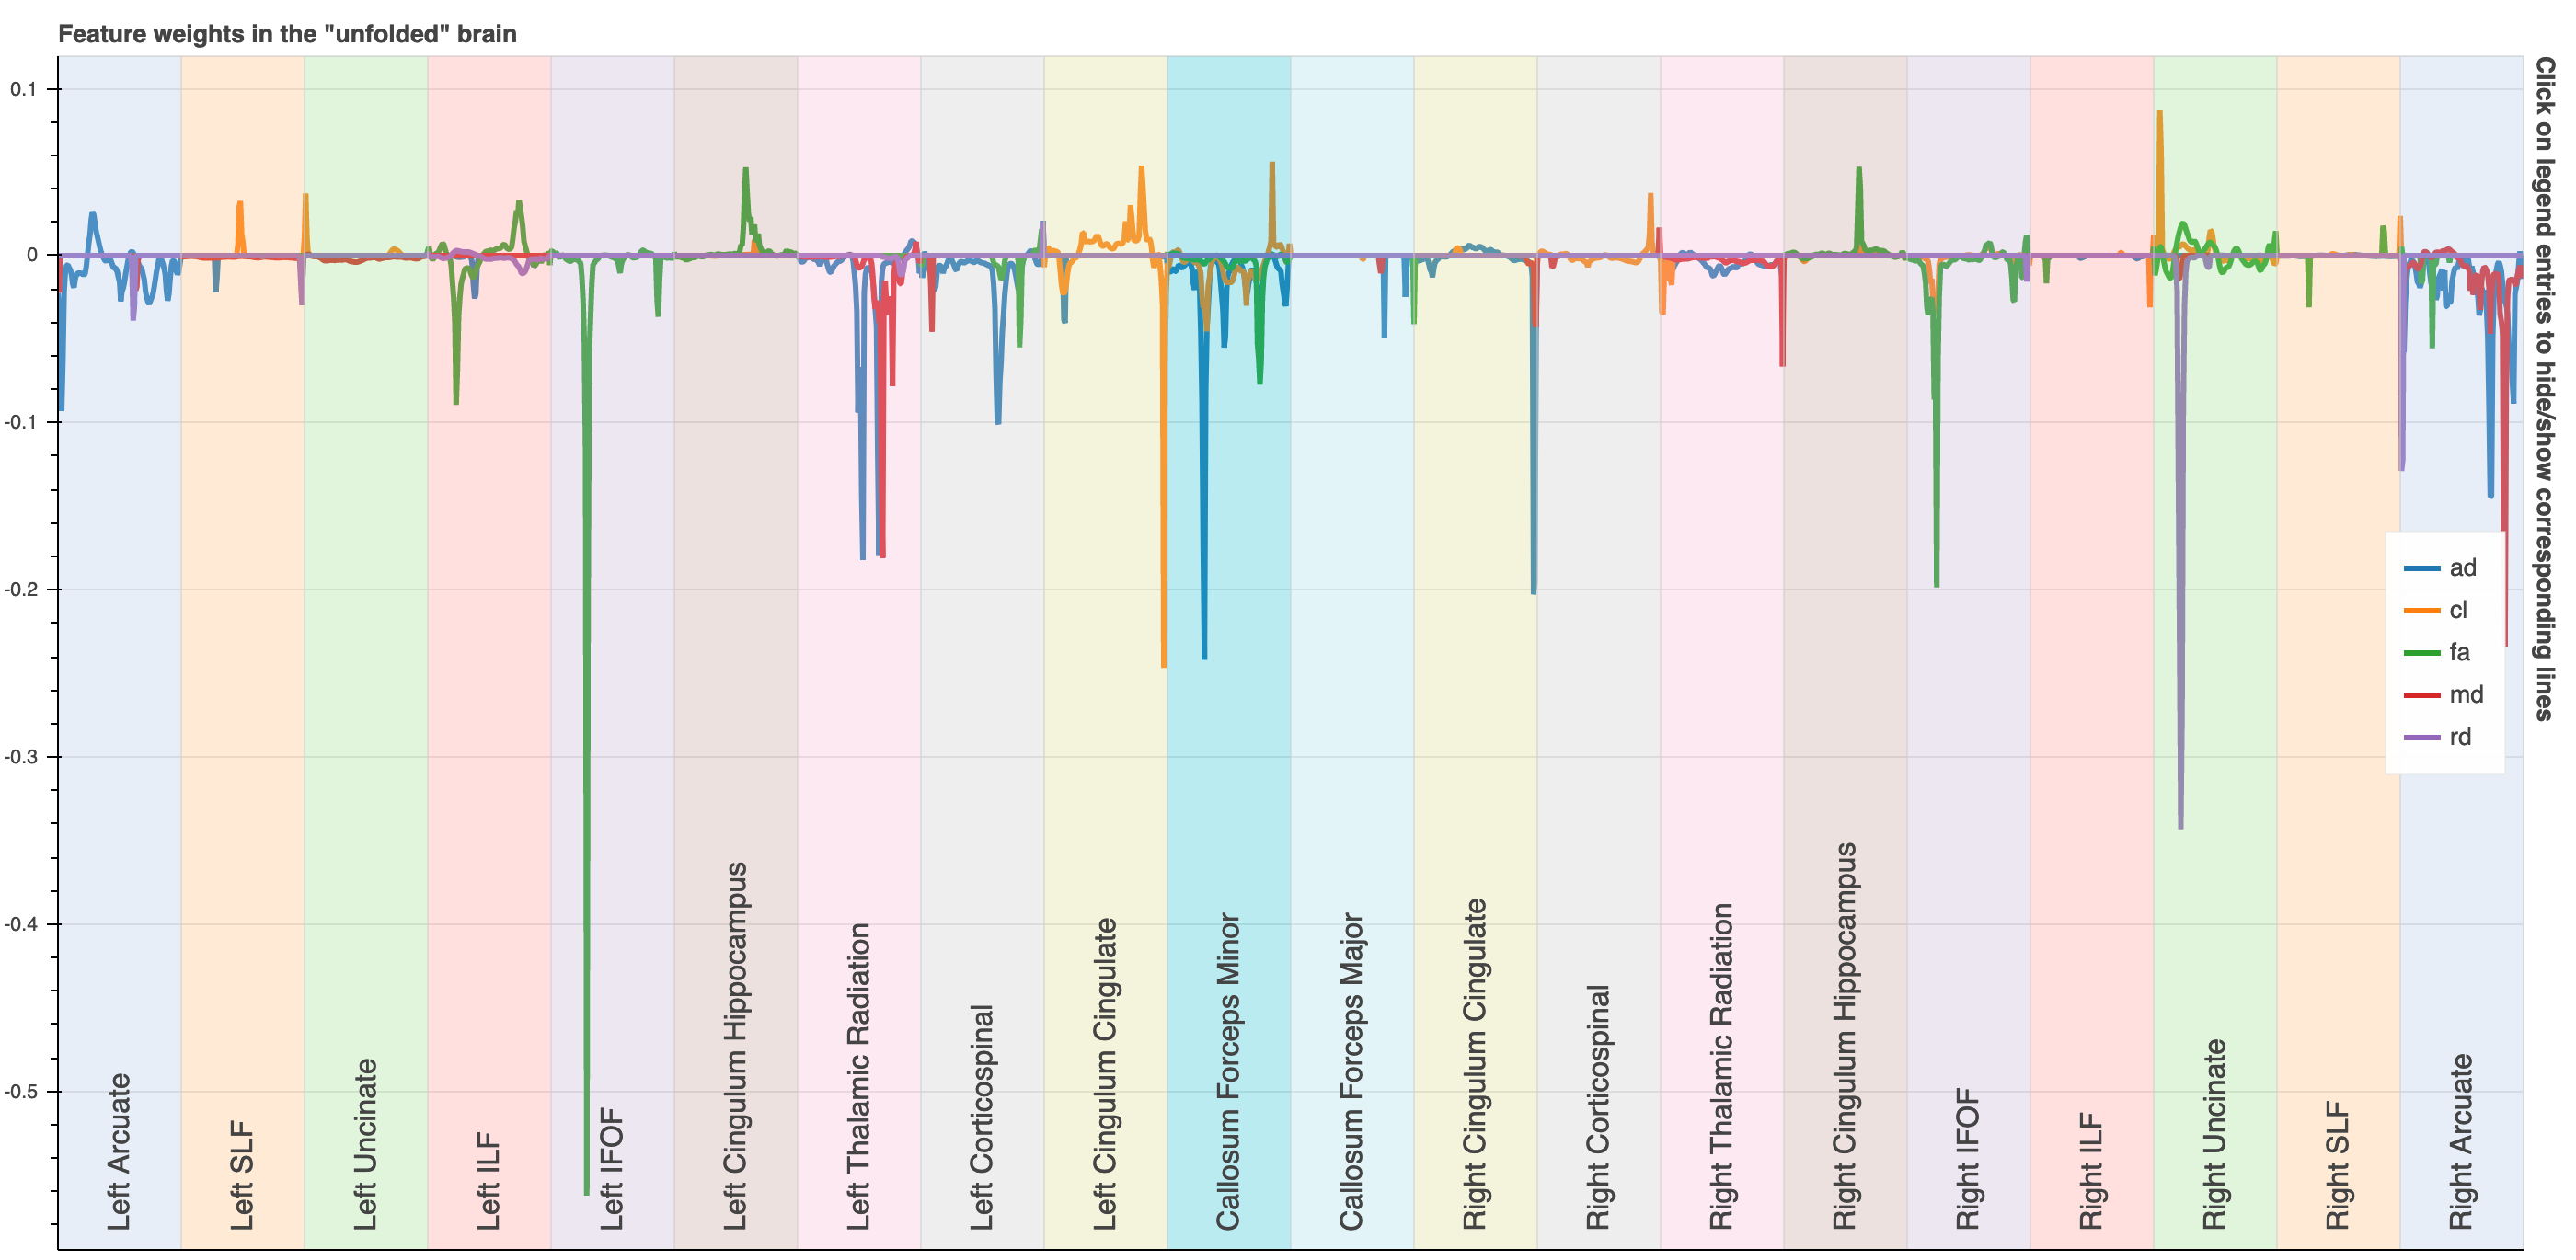
\includegraphics[width=0.95\textwidth]{regression_unfolded_beta.png}
    \caption{{\bf Feature importance for brain age.}
    }
    \label{fig:regress-beta}
\end{figure}

\begin{itemize}
  \item Regression
    \begin{itemize}
      \item Lifespan maturation age regression
      \item Insert figure showing sparsity pattern
      \item Insert figure showing weights as they relate to tract differences visible in the browser
    \end{itemize}
\end{itemize}
\begin{itemize}
  \item Failures
    \begin{itemize}
      \item Hopefully, the failures are common to both regression
        and classification so we can include them here in there own
        subsection.
      \item Insert figure demonstrating failure cases
    \end{itemize}
\end{itemize}
